\chapter{Conceptual Framing and the Ecological Turn}
\lhead{\textit{Conceptual Framing and the Ecological Turn}}

\textit{\textbf{Chapter Summary:} This chapter turns back to the research problem stated in Chapter 1, namely, to identify conceptual principles to integrate intercultural communication and ecology. It is argued that the thought of two twentieth century philosophers, Ludwig Wittgenstein and Hannah Arendt, provide rich concepts and vocabulary to this end. To help operationalize these concepts, the four levels of discourse are revisited by outlining \textit{concepts of discourse} and \textit{aims of analysis}.}
\newline

The three analyses in the preceding chapters differ vastly in terms of types of linguistic data as well as topics discussed. Analysis 1, which covers GM seed, spans different geographic locations and is concerned with nature at the molecular scale. Analyses 2 and 3, by contrast, focus more on specific times and geographic locations, at the scale of the built environment of raw materials and infrastructure. The communication data also vary widely between the analyses, from the level of whole texts (Corpus 1), to verbal utterances (Corpus 2) and, finally, nonverbal microexpressions (Corpus 3). Following these three analyses, we return to the question of what conceptual principles can guide our understanding of human communication in relation to the natural world. This present chapter integrates the analyses and begins to sketch out conceptual aspects of the topic. 

In each of the analyses, there are a complex array of issues and factors to consider. The multilevel method sheds light on the sheer breadth of these issues. If nothing else, a takeaway from the analyses is that issues at the interface of the natural environment and human cultures are complex and multifaceted. On the one hand, understanding the interface between humans and the environment requires interpretive approaches based on humanistic inquiry to grasp the experience [\textit{Erlebnis}] of what a given environmental issue means for different groups and communities. On the other, viewing issues through the lens of humanistic inquiry alone is not sufficient. Often the issues concern economics, power, and resource distribution, in which case more social scientific inquiry is called for. Beyond both humanistic and social scientific inquiry there is a crucial role for empirical science as the bedrock for understanding ecological issues. 

Thus, at the outset, we are confronted with the basic question of how to combine modes of inquiry in a way that allows for the study of the natural world alongside human cultures and communication. ICC research generally draws from social scientific or humanistic modes of inquiry \citep[see][]{Littlejohn2011a}. By contrast, any theoretical approach to the natural environment would almost certainly refer to the natural sciences. Cultural and communication studies are often based on constructionist, postmodern premises which often clash with the objective and empirical aims of the natural sciences. Without compromising the role of the scientific argumentation and empirical evidence in both understanding and addressing ecological issues, there is also a need for meaning-centred approaches to the natural world. In other words, environmental issues are not only questions about scientific evidence and theories about nature; they also concern how nature is experienced, interpreted, and is a source for meaning.

One can begin to see the need for interdisciplinary approaches. However, without shared principles and concepts, such approaches are unlikely to succeed. The question then becomes, what are unifying concepts that can serve as a departure point for understanding the interface between intercultural communication and environmental issues?

In seeking this conceptual orientation there are certain criteria that can serve as a starting point. First, it is advantageous if the approach is anti-essentialist and capable of dealing with fuzzy categories, but not at the cost of a consistent and realistic critical stance. Second, the orientation should be reflexive and modest with respect to our own epistemological position. Finally, given calls to de-westernize communication theory and discourse studies \citep[e.g.][]{Shi-xu2005a, Tapas2012a, Waisbord2014a}, a range of intellectual traditions should be considered. In short, the researcher is engaged in an open, non-reductive intercultural philosophy \citep[see][]{Mall2000a}.

By combining intercultural and ecological themes, we are grappling with two broad features of both human societies and natural systems: plurality and complexity. Plurality refers to the uniqueness and variety of cultures, languages, and lifeforms. Complexity refers to the manifold ways in which these phenomena combine, evolve, and interact. We are especially interested in how plurality and complexity are reflected and embodied in human communication. To begin to outline conceptual principles, we turn to two thinkers. The first is Ludwig Wittgenstein; notably, concepts from his later philosophy such as language games and unsurveyability. The second is Hannah Arendt, more specifically her notions of the plurality and the public sphere.

\section{Language Games}

A key question that emerges from the analyses is how to understand the varied complexities of human languages, cultures, and communication. Wittgenstein's notion of \textit{language games} is a concept that can help us understand the diversity of human communication that we encountered in the three corpus-based analyses.  

A language game can be understood as a communicative activity, with its own rules, connotations, and meanings. In the corpus data from previous chapters, different people are using language in very different ways and for different purposes. Although they speak the same language in a literal sense (i.e. English), the language games they are playing often diverge. Expressing a cultural identity is an entirely different language game than, say, making a scientific statement. Yet, such differences pervade environmental discourse. Appreciating these language games is a first step in overcoming misunderstandings. In what follows we'll discuss the idea of language game and its implications for intercultural communication. Then, we'll consider how the idea is manifested in the corpora from previous chapters.   

With his notion of language games, Wittgenstein deconstructs the deeply-seated view in the Western philosophical tradition that words correspond to essential concepts with one underlying logic. In contrast to his earlier search for an ideal language with formal unity, Wittgenstein's later work emphasizes the diversity and complexity within ordinary, everyday language. This diversity is rooted in the pluralism of the human condition and multiple ways of seeing the world (BB, 59).\footnote{Abbreviations of Wittgenstein's works: PI: Philosophical Investigations \citep{Wittgenstein1986a}, CV: Culture and Value \citep{Wittgenstein1998b}, RFGB: Remarks on Frazer's Golden Bough \citep{Wittgenstein1993a}, BB: The Blue and Brown Books \citep{Wittgenstein1998c}, Some references to the Investigations rely on alternate translations. (e.g. ``\"ubersichtliche Darstellung'' as surveyable vs. perspicuous representation.)}

Wittgenstein refers to ordinary language as consisting of a ``prodigious diversity of all the everyday language games'' (PI). Language games reflect a diversity of world pictures, meanings, and forms of life. Wittgenstein lists some possible language games including giving and obeying orders, describing an object, or giving its measurements, reporting an event, speculating about an event, etc. (PI, \S   23). These and other language games are not merely parts of language, but are themselves ``complete systems of human communication'' (BB). The word ``games'' is telling, since it points to a set of internal rules and practices that players adhere to in order for the game to have meaning. For instance, it would be nonsensical to apply the rules and practices of chess to billiards. Just so, language games have their own set of rules for coherence. Despite the term ``language,'' language games are not confined to verbal utterances; they are semiotic practices and activities wherein language often plays a central role \citep{Xanthos2019}.

\subsection{Unsurveyability}

A crucial point in the intercultural context is that in the flow of human communication we are less likely to have an overview of the given language game being played, let alone the variety of games that are possible. As a result, one can easily be led to disorientation and misunderstanding. The notion of our being embedded in a maze of language is suggested in the following passage:   

\begin{quote}
Our language can be seen as an ancient city: a maze of little streets and squares, of old and new houses, and of houses with additions from various periods; and this surrounded by a multitude of new boroughs with straight regular streets and uniform
houses. (PI, \S   18)
\end{quote}

Like a city, our language is a mosaic that is constantly changing and evolving. Moreover, we are embedded in this ``city'' and do not have one overarching map of how the various parts form a whole system. Our interface with a language game is not with the game as a whole, but the constituent parts, or ``moves.'' By consequence, we do not have an overview of language and its many uses. This lack of overview led Wittgenstein to claim ``our grammar lacks surveyability'' (PI, \S 122). Here, ``grammar'' does not refer to grammatical rules but, rather, to a ``pattern of linguistic practices'' \cite[90]{Sluga2011a}. Natural language is unsurveyable [\textit{un{\"u}bersichtlich}] such that we cannot grasp it in its entirety. 

For something to be unsurveyable implies that it can be described and expressed but not fully explained. Insofar as natural language can serve as a tool for description and expression, its complexity and diversity is homologous to that of forms of life. It follows that we can think and speak of these complexities not by reference to external criteria or truth, but only based on our own phenomenological experience. That is, through metaphor, analogy, and ``connection[s] with our own feelings and thoughts'' (RFGB, 143).

When attempting to understand complex phenomena like cultures, surveyability is fundamental since it is precisely our predefined conceptual schema or ``the way we look at things'' that ``earmarks the form of account we give'' (PI, \S   122). Surveyable representation is therapy for the conceptual problems that ensue as a result of a craving for universal laws and explanations. Wittgenstein's work can be the basis of cultural metacritique, providing critical awareness of the tendency to apply overly reductive, narrow approaches to unsurveyable human phenomena. The metacritique would apply in situations where the complexities of culture and communication are not fully acknowledged.

The unsurveyability of cultures does not preclude intercultural understanding. To the contrary, human understanding is always possible since, even when language games and actions are part of different cultures, they are rooted in ``shared human behaviour'' that constitutes ``the system of reference by means of which we interpret an unknown language'' (PI, \S   206). As a result, the diversity of cultures and world pictures are mutually intelligible. Even if we are unable to obtain a surveyable representation of cultures, we can begin to understand their form of life through metaphors and analogies of that which is familiar to us. We can observe particulars and begin to see how they form an interconnected whole.

The idea of unsurveyability refers to our inability to obtain a comprehensive and objective view of complex human phenomena such as cultures. It helps us maintain a critical awareness of the tendency to apply overly reductive, narrow approaches to the complexities of human communication. Beyond mere critique, the idea of language games might help resolve misunderstandings. Communicative misunderstandings can be understood as the result of incompatible language games both within and between cultures. The challenge for discourse analyses (such as those in the previous chapters) might be distinguishing the possible language games taking place. This involves description and analysis of diverse and overlapping systems of communication; that is, describing rules that guide the speech and behaviour, the meanings of words within a system of reference, the human needs that the language games fulfill, and actions to which they correspond. Holding up these descriptions in parallel, one might begin to see fissures and connections between them which, ideally, would help overcome misunderstandings. 

\subsection{Cultural Language Games}

Wittgenstein's thought can serve as a reminder of how to approach the very idea of culture. The concept of culture is elusive; it is often uncertain what, precisely, we are referring to as \textit{cultural}. Given that uncertainty leads to stress responses in humans \citep{DeBerker2016}, it is natural to seek more secure conceptual ground by approaching issues through more clear and distinct frameworks. But to paraphrase from Wittgenstein's \textit{Philosophical Investigations}, is an indistinct concept not ``often exactly what we need?'' (\S 71). To refer to culture as an ``indistinct concept'' is to say it has a cluster of meanings and associations. It is complex, multilayered, and unsurveyable. Culture can refer to a myriad of subjective experiences, artifacts, behaviors, practices, beliefs, values, communication patterns, cognitive structures, etc., so vast and complex as to evade sharp definition.

The multilevel framework introduced in Chapter 2, rests on the premise that cultural discourse is distinguishable from other discourses. We can view discourses as consisting of language games that are ``culturally infiltrated'' to varying degrees \citep[5]{Shi-xu2005a}. In this section, we expand on the idea of cultural discourse by referring to examples from the corpora. Based on the cultural-level of analysis, we can propose some elements of cultural language games as the following: 

\begin{itemize}
    \item Communicative interactants are engaging in commentary about who they are, their worldviews, values, and identities  \citep[see][]{Carbaugh2007a}.
    \item Meanings are expressed with a high degree of connotation and symbolism. 
    \item They invoke internal emotions and mental states while, simultaneously, expressing connections beyond the self. These expressed connections are most often to a group of people/community, but might also refer to place, or the natural world.  
\end{itemize}

In previous chapters, we also see how cultural discourses coincide with other language games. Often, various participants in the discourse fails to acknowledge or understand that multiple language games are taking place. In all three corpus-based analyses, it is common to see participants `speaking past one another', where the language game employed by one participant in the discourse is incompatible with another.  

In Chapter 3, we see a plurality of overlapping language games (economic, political, ecological, cultural, etc.) within the GM seed debate. This plurality renders anti-GM discourse as a whole difficult to grasp and susceptible to misunderstanding. The pro-GM side of the discourse uses language to make claims about facts or states of affairs in the material world. The preconditions and assumptions underlying these facts are tightly defined. For instance, consider the statement:

\begin{footnotesize}
\begin{quote}
\texttt{Many GMOs are tailored for specific environmental conditions, which means saving water in drought-prone areas and less use of chemicals.}
\end{quote}
\end{footnotesize}

Another speaker can challenge this statement whilst still `playing' the same language game. For example, an anti-GM speaker might respond by asserting that non-GM and organic methods of production are less water intensive and use less pesticides than GM production. This counter argument adheres to the implicit rules and aims of the original; that is, to make an objective claim about water and pesticide use. However, consider that someone responds to the a claim that GMOs use less water and pesticides by saying the following:

\begin{footnotesize}
\begin{quote}
\texttt{[]But] if Paraguay is so dependent [on foreign companies] for such a basic thing as food...it means that this is a subordinate country.}
\end{quote}
\end{footnotesize}

Here, the language game is entirely different. It is no longer concerned (at least primarily) with making objective fact claims about the material world, it is now a hypothetical statement. Moreover, the hypothetical introduces non-material concepts like dependency, subordination, and national sovereignty. For a meaningful discussion or debate to ensue, both interlocutors would have to be aware of the context and issues. This second statement begins to take on a cultural dimension, in that national identity is expressed vis-\`a-vis the power of foreign companies. However, it might more appropriately be described as a political-economic (as opposed to cultural) language game. By comparison, the following statement (also from the GM seed corpus) is more explicitly cultural: 

\begin{footnotesize}
\begin{quote}
\texttt{The imposition of transnational frankenseeds would mean an end to this richness and the loss of the ancestral milpa tradition as a sustainable system of maize production and symbol of the Mesoamerican cultural inheritance.}
\end{quote}
\end{footnotesize}

Here, we see the elements of cultural language games: commentary about identity (Mesoamerican indigenous culture); connotative meaning and symbolism (maize as a symbol, ``frankenseeds''); and an internal mental state (``richness'') together with group connection (producers, ancestry, inheritance). A cultural language game is being played and to coherently take part in this game, one would need to engage with analogous concepts an emic understanding of the cultural connotations. To respond to this cultural language game with a statement about material fact (as in the first quotation above) would be meaningless.

Granted, these are isolated examples from a corpus and not real exchanges in the flow of a debate or conversation. Nonetheless, much of the GM seed debate functions in this way: that is, statements are made which often do not account for the context and meanings that the other `side' is operating on.  

\subsection{Language Games of Culture \& Civilization}

In Chapter 4 (Analysis 2) we also see clear manifestations of cultural language games. Recall how in Analysis 2, statements are grouped. Group A consists of pipeline proponents (or those critical of protestors), Group B are statements by pipeline opponents that were political-economic in nature, and Group C consists of statements by opponents that were deemed cultural. In the ecological-level of analysis, we observe that the theme of culture only begins to emerge in Groups B or C. Cultural groups are scarcely mentioned in Group A. This observation raises the question of whether language games can be devoid of culture.  
 
The multilevel framework introduced in Chapter 2 is based on the need to distinguish culture from other levels of analysis, such as socio-economic factors. In this section, we can expand on that distinction to discuss the differences between culture and civilization, which was mentioned in earlier chapters but not fully elaborated. The distinction between culture and civilization can be traced to Oswald Spengler's \textit{Decline of the West} as well as more recent interpretations of Wittgenstein \citep{Cavell1988a, Cavell2013a, DeAngelis2007a}. The difference is also alluded to in the German term \textit{Zivilisation} referring to an ``outer'' shell of human experience, with \textit{Kultur} as the inner essence \citep[11]{Botz-Bornstein2012a}.

To better understand this distinction in the context of language games, we can briefly turn to the influence of Oswald Spengler on Wittgenstein's thought. As opposed to a linear view of history and progress, Spengler depicts an organic birth and death, waxing and waning of cultures culminating in their decline as civilizations. Civilization is the exhausted, final stage of culture. The following passage from \textit{Decline of the West} depicts the death of culture in civilization:

\begin{quote}
Civilizations are the most external and artificial states of which a species of developed humanity is capable. They are a conclusion...death following life, rigidity following expansion, petrifying world-city following mother-earth.... The world-city means cosmopolitanism in place of ``home.'' \cite[24-25]{Spengler1965a}
\end{quote}

An analogous view of culture and civilization can be found in Wittgenstein's notebooks:

\begin{quote}
It is very remarkable, that we should be inclined to think of civilization -- houses, trees, cars, etc. -- as separating man from his origins, from what is lofty and eternal, etc. Our civilized environment, along with its trees and plants, strikes us then as though it were cheaply wrapped in cellophane and isolated from everything great, from God, as it were. That is a remarkable picture that intrudes on us. (CV, 50).

Perhaps one day a culture will arise out of this civilization. (CV, 74)
\end{quote}

Secondary interpretations tell us more about the concepts of culture and civilization that are implicit in these passages. Notably, Cavell (\citeyear{Cavell1988a,Cavell2013a}) claims that Wittgenstein's work is in response to the Spenglerian cultural decline in the modern age. Specifically, Cavell claims that ``Wittgenstein diurnalizes Spengler's vision of the destiny toward exhausted forms, toward nomadism, toward the loss of culture, or say of home, or say community'' (262). According to this interpretation, Wittgenstein views the language of civilization as externalized from the language games and form of life from which it developed. Speaking outside language-games is ``homologous'' to the ``decline of culture as a process of externalization'' \citep[261]{Cavell1988a}. In referring questions of philosophy back to ordinary language, Wittgenstein is ``forgoing, rebuking, parodying philosophy's claim to privileged perspective on its culture, call it the perspective of reason (perhaps shared with science)'' \citep[263]{Cavell1988a}.

For \cite{Lurie1989a} this lament of civilization as the ``taming of Nature and man'' aligns Wittgenstein's thinking with the Romantic movement (378-379). Similarly, for \cite{Pradhan2000a}, Wittgenstein is expressing how ``twentieth century materialist civilization'' has become ``detached from the springs of life and soul'' (110). \cite{Cerbone2013a} claims that Wittgenstein is commenting on ``something distinctively \textit{inorganic} about how human beings live,'' analogous to his philosophy ``on the \textit{organic} and \textit{living} character of language'' (255, original emphasis). Finally, \cite{Rudd2013a} refers to Wittgenstein as a ``Romantic modernist'' who sought to deconstruct a way of thinking that crowds out spirit, expression, and wonder (233-234). 

Granted, this interpretation may seem speculative and somewhat disconnected from the present study. Therefore, we return to Analysis 2 for insight into how the culture/civilization distinction functions in the practice of human communication. The contrast between Groups A and C might be seen as an embodiment of the contrast between civilization and culture, respectively. As Figure 6.1 indicates, themes in Group A mainly concern mechanisms of social organization such as law, administration, and security. Group A contains several references to payment, private property, and monetary value. By contrast, Group C is full of religious and spiritual terms, including \textit{sacred}, \textit{spiritual}, and \textit{prayer}. Another notable difference is the time horizon imminent in the communication. While Group A largely focused on immediate events, in Group C it is common to refer to multiple generations or invoke the historical context.

\begin{figure}[H]
\centering
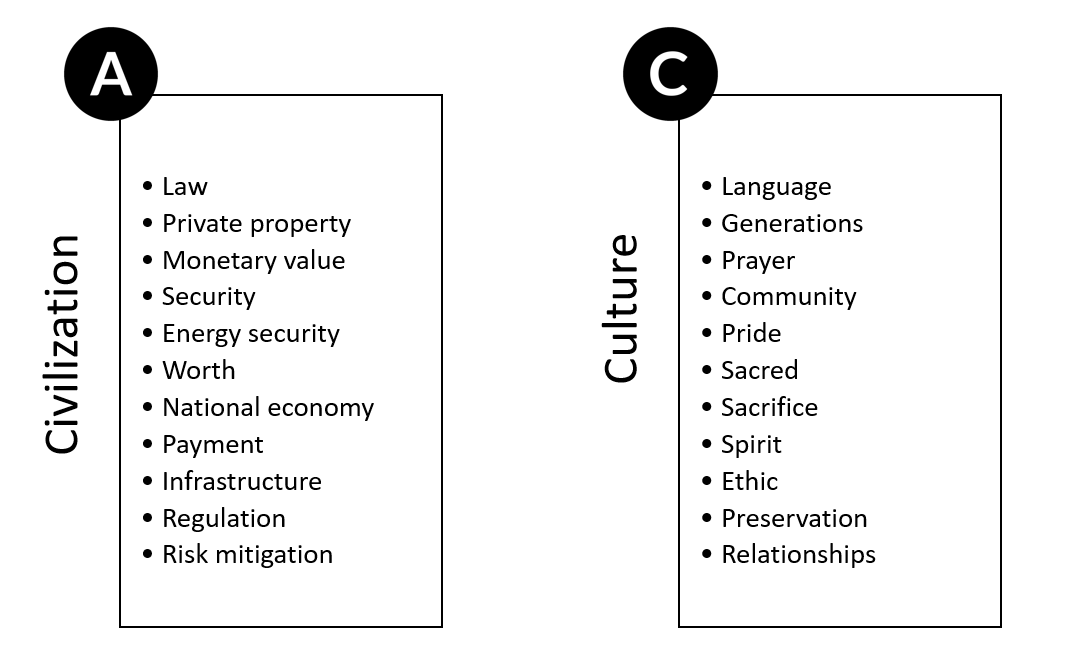
\includegraphics[width=10cm]{Figures/groupcontrast.png}
\caption{Key themes from Groups A and C in Analysis 2 (Chapter 4)}
\label{fig:figure1}
\end{figure}

Given the standpoint of the speakers, the contrast between A and C is not surprising. While those in Group C are speaking as members of civil society or communities, Group A is made up largely of individuals acting in occupational roles, representing state institutions or corporations. Arguably, speakers in Group A are compelled to employ relatively narrow discourses or `talking points'. In this sense, the two groups are playing entirely different language games. 

Between A and C, is Group B, where pipeline opponents invoke notions of trust, fairness, and inequality. Speakers in Group B speak out against an oppressive justice system, corporate power, exclusion, and economic inequality. Group B offers counter discourses to Group A. Speakers are engaging in critical commentary of broader social and institutional structures. In other words, they are expressing malaise with the prevailing civilization. While there are references to cultural groups, these are most often in the context of broken promises and perceived bias; these are not affirmative expressions of cultural identity in the same way as Group C. In terms of cultural discourse, the three groups can be summarized as follows: 

\begin{itemize}
  \item \textbf{Group A} consists of acultural statements representing social/institutional structures.
  \item \textbf{Group B} consists of statements made in reactive opposition to Group A, or challenging the legitimacy of A.
  \item \textbf{Group C} consists of affirmative assertions of culture.
\end{itemize} 
  
Group B is playing a language game compatible with A (call it a language game of civilization or institutions). At the same time, however, speakers are making some cultural assertions related to their identities and values. In this sense, Group B is also a pivot away from the language game of A. The malaise expressed in Group B can be understood as a move towards cultural assertions observed in Group C. Cultural discourse is thus conceived as a turning away from the language games of institutional power structures. Lost of trust and legitimacy with respect to the wider society is restored by a turn toward shared identity and experience.  
 
A similar grouping can be considered in Chapter 5. Here, we note how nonverbal communication operates differently depending on the level of discourse. Nonverbal expressions and their cognitive underpinnings are tied up with a given language game. Cultural language games are often accompanied by expressions of pride, confidence, and empowerment. Like Group C in Analysis 2, the cultural-level statements in Analysis 3 are affirmative. The socio-economic statements, on the other hand, are made in resistance. Rather than affirmative stances, speakers are speaking from a position of vulnerability and even fear. This contrast suggests that the language games operate beyond the content of verbal expressions, and are bound up with cognition and behavior.    
 
Following the argument that cultural language games are distinct from those of civilization, we can consider the aims for discourse analysis. One such aim might be to point out and resist departures from culture in the name of civilization or material progress, where ``civilization'' and ``progress'' do not refer to some more advanced state, but to prevailing ideas or myths of modern societies \citep[e.g.][]{Pollard1971a, Bowden2011a}. This aim entails the preservation of culture against onslaughts in the name of social or economic progress. From a critical standpoint, one could counter this aim, claiming it is suggestive of romantic conservatism or is reactionary to progress. However, it is possible that critical, anti-oppression, emancipatory frameworks are consistent with, perhaps even strengthened by, the idea cultural preservation. Similarly, the notion of an affirmative cultural identity as empowering could be the basis of autonomy in the face of oppression. 

Making a distinction between culture and civilization does not imply that we replace nuance and historical particularity with what could be criticised as a sweeping, Spenglerian narrative. It does, however, imply more measured use of the term `culture'. It is possible that this distinction enriches our understanding of what human cultures are and what they are not. In the contemporary context of global migrations and mass communication, contrasts between discourses of culture and those of civilization could be made; the former being expressive, symbolic, and related to dwelling in a particular time and place; the latter placeless, material, and uprooted from shared meaning. This distinction would challenge the notion of interculturality as internationalization of trade, science, technology, and socioeconomic structures \citep[see][5]{Mall2000a}. Accordingly, in societies often described as `multicultural', much of the discourse of business, media, politics, and science might be more aptly characterized as acultural cosmopolitanism. 

\subsection{Language Games \& Organicism}

The notion of language games emphasizes the diversity of human experiences, world pictures, and ways of using language. If communication is made up of sub-systems or ``games'' then one could raise the question of how mutual understanding is even possible. Underlying the diversity of language games, however, is a shared human form of life. Arguably, our shared life-form is itself constrained by the pre-linguistic, natural world. The relation to the natural world, as expressed in cultural language games, is not one of strict correspondence or \textit{a priori} understanding but is built upon layers of analogy and metaphor. The organic nature of human language has implications for the idea and aims of the ecological level of discourse analysis as well as how scientific statements can be approached in a discourse analytic framework (implications which will be elaborated in a subsequent section).

In a metaphorical sense, culture stands in relation to nature as an organic form. Organic form has a number of overlapping connotations related to artistic expression, human culture, and biological life. As a literary term, it is associated with Coleridge's idea of ``unity in multeity.'' Goethe's morphology is also ``a science of organic forms'' which aims to discover ``unity in the vast diversity of plants and animals'' \citep[xvi]{Miller2009a}. In \textit{Decline of the West}, \cite{Spengler1965a} refers to cultures through world history as the ``waxing and waning of organic forms'' (17-18).

The idea of language as organic form is embedded in the notion of language games. In later writings, Wittgenstein sees language as consisting of ``an inorganic part, the handling of signs'' and ``an organic part...understanding these signs, meaning them, interpreting them, thinking'' (BB, p. 4). The Investigations further develops the organic notion of language: ``In use it is alive'' (PI, \S 432). It is dynamic, with parts dying off and others ``coming into existence'' (PI, \S 23).

The connection between culture and organic form is based on a certain interpretation of \textit{forms of life}. Underlying the diversity of cultural language games is a shared human form of life. There are several interpretations of the meaning of this concept including social, cultural, behavioural, and biological accounts. Forms of life can be understood as patterns and regularities ``in the fabric of human existence on earth'' \citep[132]{Pitkin1985a}. \cite*{Sluga2011a} describes Wittgenstein's philosophy as a kind of naturalism where ``forms of life, worldviews, and language games are ultimately constrained by the nature of the world'' (12-13). However, one could also argue that these constraints are more anthropological than biological. \cite{Keith2012a}, for instance, claims Wittgenstein's position is one where there are no natural constraints on what can count as truth ``unless they are constraints on our shared forms of living'' (487). \cite{Cavell2013a} allows for both perspectives, suggesting forms of life be seen as a relativistic ``sense of agreement'' as well as in a more fixed, biological sense (41-42). It follows that, our shared human lifeform is itself constrained by the prelinguistic, natural world. This relation to the natural world is not one of strict correspondence or a priori understanding but is built upon layers of analogy and metaphor. 

If forms of life are indeed constrained by the nature of the world, then there would be a unifying ``system of reference'' common to all human cultures (PI, \S 206). What is common to all cultures might be activities of eating, drinking, or speaking a language (PI, \S 25). Science and technology might also reflect transcultural, universal truths. Relativistic interpretations of forms of life counter any suggestion of universalism. However, it is important to consider that Wittgenstein does not deny the possibility of a single or universal form of life. Sluga (2011) discusses a ``single form of life'' as a homogenized, unified language game and claims that, according to Wittgenstein, such a life-form would be ``impoverished and almost sub-human'' (61). Insofar as Wittgenstein invokes this possibility, it seems to have been a source of deep pessimism concerning the age in which he lived. Broadly speaking, this pessimism seems directed toward the scientism, positivism, and materialism he sees as characteristic of modern thought. As the antithesis of the organic diversity of language games and forms of life, Wittgenstein is critical of the homogenizing force of modern science and technology:

\begin{quote}
Perhaps science and industry, having caused infinite misery in the process, will unite the world\textemdash I mean condense it into a single unit, though one in which peace is the last thing that will find a home. (CV, 63)  
\end{quote}

\begin{quote}
Science: enrichment \& impoverishment. The one method elbows all others aside. Compared with this they all seem paltry, preliminary stages at best.  (CV, 70)  
\end{quote}

\begin{quote}
The use of the word ``science'' for ``everything that can be said without nonsense'' already betrays this overestimation. For this amounts in reality to dividing utterances into two classes: good \& bad; \& the danger is already there. It is similar to dividing all animals, plants \& rocks into the useful \& the harmful. (CV, 71) 
\end{quote}

These statements do not imply that Wittgenstein was somehow against science. Rather, they are a critique of the notion that the methods and aims of science can (or should) be applied across the range of human thought and forms of life \citep{Read2016}. This criticism is based on a naturalism that seeks complexity and interconnection while resisting reductionism. Similarly, an intercultural discourse analysis might aim to critique reductionism and scientism. This point returns to a previous question of how scientific statements are accounted for in a multilevel discourse framework. Critical analysis of natural scientific discourse is not directed at science \textit{per se}; rather, the ideology of scientism is what is problematic from an intercultural communication standpoint. 

Organic form functions as an ontological metaphor \cite[25]{Lakoff1980a}, whereby our experience of lifeforms is the basis for understanding. For example, we can consider how Coleridge identified organicism in properties of the plant. These properties are explained as five principles by \citeauthor{Abrams1953a} (\citeyear[170-75]{Abrams1953a}). These principles (and the organic form metaphor) might be extended to human cultures as follows:

\begin{enumerate}[i.]
  \item \textit{The whole is prior to the parts}. Although cultures are made up of a multitude of parts (people, groups, practices, beliefs, etc.), the culture itself is irreducible and cannot be understood through individual components separate from the whole.
  \item \textit{The process of growth is conveyed}. Growth as ``the first power'' of living things is manifest in cultures. Human cultures are dynamic, undergoing growth, death, and evolution. 
  \item \textit{Diverse elements are assimilated into the whole}. Human cultures form as individuals and groups combine. The individual elements metamorphize into the whole.
  \item \textit{Form and growth is directed from within}. Cultures evolve spontaneously from within. By contrast, mechanical forms arise through an externally imposed structure.
  \item \textit{Unity in multeity}. In human cultures, a complex interdependency of parts forms a whole. The whole and parts are interdependent, with the whole (culture) relying on the components and vice versa. 
\end{enumerate}

The organic form metaphor for cultures is consistent with an antireductionist and holistic approach that, in the opening of this chapter, was stated as necessary for intercultural research. Nature, as the organic wellspring for cultures, consists of complex forms of life. It follows that culturally imbued statements themselves evoke this complexity which, while expressed through cultural practices, may not be articulated or rationalized.	

\section{Unsurveyability \& Cognitive Bias}
 
The previous discussion deals with philosophical concepts that, one could argue, do not clearly apply to the everyday practice of intercultural communication. In order to sketch out how these concepts might be applied, this section discusses the idea of unsurveyability in terms of cognitive bias. The argument is that, in the three analyses of environmental communication, there is a tendency to move away from the cultural context, towards more defined, measurable ways of framing the topic. This tendency can be seen as a natural cognitive response in the face of complex, unsurveyable phenomena.   

Culture and communication are what \cite*{Sluga2011a} terms ``hyper-complexities'' (146). At most, we can only obtain partial understandings of the language games and multilevel interactions that constitute a given discourse. In the face of complexity, it is natural to reduce and categorize. For instance, from the some 7.5 million colours discernable by the human eye, we assign categories like red, glue, green, etc. \citep[889]{Hinner2017a}. This categorization prevents chaos in the realm of human perception and cognition, allowing us to simplify phenomena to manageable proportions. However, this inherent tendency to simplify and categorize can lead to bias. Cognitive bias arises from heuristics and mental shortcuts in the face of uncertainty and complexity \citep{Kahneman2002a}. Bias may thus be understood as information-processing shortcuts in the face of uncertainty \citep{Tversky1974a} or noisy information \citep{Hilbert2012a}, together with the human brain's limited capacity to process that information \citep{Simon1955a}.

Culture is a hyper-complexity with layers of metaphor and meaning inherent in behaviors and utterances. For example, in the corpus examples we see how cultural statements evoke connotative, contextual, and figurative meanings \citep{Klopf1998a}. Yet, in the face of this complexity it is common for people to frame discourse in narrower, more literal, and more sharply defined terms. This framing often negates the cultural context. This turn away from complexity might be described as a \textit{surveyablity bias} whereby, in the face of complex unsurveyable phenomena, people frame the issue according to a limited perspective. Like other biases, the surveyability bias can be viewed as a mental shortcut in the face of complexity. Unlike the conventional notion of bias as prejudice, surveyability bias is a departure from cultural meanings altogether. For instance, in the GM seed debate which (as we note in Analysis 1) is highly cultural, there is a narrowing of the discourse to issues of safety and efficiency. Due to the complexity of cultural schemas, there is an inherent tendency to perceive and interpret that which is part of the common system of reference while neglecting the culturally variant frame. 

This notion of bias changes the way we might look at intercultural misunderstandings. In intercultural encounters, it is common to refer to cultural bias, which is a preference for one cultural group over another \citep{Yingst2011a}. Similarly, intercultural conflict is conventionally seen as a perceived incompatibility between different cultural communities \citep{TingToomeyS}. However, many conflicts between groups are not intercultural. Likewise, communication from people from different cultural communities often does not necessarily lead to misunderstanding. Rather than looking at how conflict arises from differences among cultural groups, it may be more appropriate to view conflict and misunderstanding in terms of whether the cultural dynamics are even being taken into account. In modern, pluralistic societies people do not express their cultural identities at every turn, at least in the public sphere. In terms of the familiar culture as an iceberg metaphor \citep{Hall1973a,Hall1976a}, daily lives are conducted at the surface. As opposed to viewing communicative interactions as encounters between different cultures, we can consider how culture emerges to the surface at different points.	 

As discussed, human communication can be viewed as an amalgam of different language games. Different language games imply different rules that guide the speech and behaviour; different meanings of words within a system of reference; different human needs that the language game fulfils; and actions to which it corresponds. Along these lines, communicative misunderstandings result from incompatible language games both within and between cultures \citep[10]{Frayne2017a}. More specifically, misunderstandings result when interactants are unaware that entirely different language games are being played. Surveyability bias is precisely this lack of awareness that a language game is indeed cultural.

\subsection{Family Resemblances \& Surveyability Bias}

Like other biases, the surveyability bias is unavoidable and part of our cognitive make up. However, there are certain ways of thinking that can counteract this bias. The remedy for surveyability bias is to obtain a more synoptic view or surveyable representation of complex phenomana like cultures. This ``consists in seeing connections'' (PI, \S 122). Wittgenstein claimed ``our grammar lacks surveyability'' (PI, \S 122), implying the complexity of natural language is such that we cannot grasp it in its entirety. Even though we cannot represent language as a whole system, we can look at its multiple uses. Taken together, these particular uses will reveal relations and patterns of similarities that can be characterized as ``family resemblances'' (PI, \S 67). Family resemblance is a way to confront the challenge of understanding cultures, their language games, and the set of relations that exist within and between them.

Rather than serving as an entirely new idea, family resemblance gives new expression to what is already implied in much intercultural research, particularly comparative approaches. Like language games, cultures can be characterized as having both intercultural and intracultural family resemblances. In other words, when we associate people or things with a culture X, we are saying there is ``no one thing in common which makes us use the same word for all'' but that they are related ``in many different ways'' through ``a complicated network of similarities overlapping and criss-crossing'' (PI, \S 65, 66). In the same way, different cultures form a complicated network. Amid the plurality of cultures and language games, interconnectedness makes communication and understanding possible. Family resemblance need not imply strict biological inheritance. By contrast, it is a general picture that forms when any number of individuals/entities are grouped together by a set of characteristics that may not be common to all \citep{Ginzburg2004a}. Networks of biological descent, family bonds, ethnicities, races and nations might be an important part of this grouping. However, there are other important factors such as citizenship, geography, or shared history \citep{Sluga2011a}. Establishing family resemblance is a matter of sketching out the multiple relationships. The task for intercultural research could be to form a ``genealogy of concepts'' within and between cultures \citep{Canfield1993a}. In this, metaphor and analogy are central since it is in this way that cultures relate back to a shared human form of life.

In Analysis 1, we see examples of the role of metaphor in maintaining agreement and mutual understanding among anti-GM critics. In the keywords, concordances, and the ``Maize Manifesto'' excerpt, there is a bidirectional metaphor between culture and nature. In other words, there is an implicitly understood reciprocal relationship between human culture and nature. The diversity and complexity of each is understood in terms of the other. The function of this biocultural metaphor is to capture the internal complexity of the topic at hand and frame the issue holistically. Thus, even if GM critics do not share a common culture, there is a common set of concepts that create meaning and reconciles worldviews cross-culturally.  

The pipeline debate (Analysis 2) also has a strong cultural element, particularly with respect to the indigenous groups. Here, we see the expression of cultural values, or a set of deeply held beliefs among a cultural group \citep[95]{Martin2010a}. However, non-indigenous voices are also present. We see family resemblances between these different worldviews with respect to, for instance, the spiritual dimensions of nature.

In the three analyses we observe that disagreement and misunderstanding arise from the inability to make connections between worldviews and experiences, not necessarily from cultural differences. At times the source of disagreement is ontological, insofar as it related to underlying assumptions about the nature of reality and categories of being. At other times, the disagreement could best be traced to cognitive factors, in the sense that it goes beyond ontological thinking to also encompass values and emotions \citep[114]{Palmer1996}. 

What we observe from the three analyses is that environmental issues bring clashes and contrasts in worldviews to the forefront. Of course, environmental issues are not unique in this regard. However, there are few topics that expose, like environmental issues do, that worldviews differ even with respect to the human understanding of the natural world. In other words, whereas we might often attribute differing worldviews to subjective interpretations, environmental debates remind us that worldviews operate at the deeper layer of the ontological and epistemological approaches to nature itself.

To summarize, Wittgenstein's thought can help us conceptualize the relation between culture and language. Concepts of language games and unsurveyability allow us to grasp the challenges of understanding one another. We can consider the notion of family resemblance as a framework for overcoming these challenges. For intercultural research, we might also consider the idea that there are discourses of culture and civilization. Implicit in this latter point is that discourses of culture are rich and meaningful in ways that those of civilization are not. This discussion leads to the question of the conditions under which mutually intelligible cultural language games are made possible. To address this, we turn to the idea of the public sphere.

\section{Plurality \& the Public Sphere}

Concepts form Wittgenstein's philosophy help us integrate culture, communication, and language. One potential drawback of these concepts, however, is that have relatively little to say about the political sphere or the socio-economic level of analysis. To account for this, another point of departure for a non-essentialized conception of intercultural communication are Arendt's notions of plurality and the public sphere. Arendt's thought can be placed within the phenomenological and hermeneutic traditions; the former rooted in direct engagement with the world and the latter concerned with interpretation of meaning. Since it emphasizes language and social interaction, hermeneutic phenomenology is especially relevant to communication theory \citep[49]{Littlejohn2011a}. Its emphasis on language as a conduit of meaning also makes this tradition relevant to intercultural understanding.

Plurality is based on the premise that ``nobody is ever the same as anyone else who ever lived, lives, or will live'' \citep[78]{Arendt1958a}. A plurality of perspectives emerges from the radical finitude of each human having been born into a unique place and time. However, this is not an individualized or atomized existence. Our being-in-the-world is characterized by a ``web'' of human relationships within which we experience this plurality \citep[175]{Arendt1958a}. This plurality ``is a blessing'' since the perspective of the others puts one's own perspective ``in relation with the world'' \citep[443]{Gambetti2005}. In the condition of plurality, humans come together and deliberate through the public sphere. The public sphere has the capacity to unite humans in meaningful action while preserving their freedom and plurality. 

Arendt's notions of plurality and the public sphere are pertinent to environmental communication. As the three prior analyses highlight, ecological issues are debated in diverse societies across multiple, unbounded geographic scales. These discourses take place in similarly unbounded intercultural communicative spaces that can be described as the ``global public sphere'' \citep{Volkmer2014}. Deliberations about environmental issues constitute what Arendt described as the two dimensions of the public sphere: (i) the \textit{space of appearance} and (ii) the \textit{common world} \citep{DEntreves2018a}. In an age when political processes are privatized \citep{Wolin2008}; civic institutions eroded \citep[see][]{Putnam1995}; and digital communication commodified \citep{Fuchs2009a}, the physical environment becomes a \textit{space of appearance} for authentic and free deliberation. Moreover, since environmental issues speak to the basic necessities of life (water, food, air, etc.) they are crosscutting themes in pluralistic societies. Amid all the planet's cultural diversity, the earth itself is a basis for common action. The environment is the ground upon which the \textit{common world} of human artifacts and institutions is established.

Arendt's public sphere theory points to the importance of maintaining conditions for free and open discourse. A challenge for pluralistic societies is not only misunderstandings and conflicts that arise within the public sphere due to, for instance, intercultural differences. The challenge also lies in creating and maintaining spaces where free and open communication can even take place. The very spaces that allow for public deliberation are often influenced and thwarted by dominant groups and ideologies in society. Structural and institutional forces can undermine the open and pluralistic character of public spaces. In modern capitalism, these forces often stem from economic interests or the harnessing of political institutions to advance private ends. If we take Arendt's notion of the public sphere as a prerequisite for intercultural communication, then crucial questions for ICC research relate to the political and economic conditions that impede authentic communication from taking place.

Another important question for ICC is the role and influence of scientific discourses in the public sphere. Of course, in the context of environmental issues, there is an indisputable role for scientific discourse to play. However, science is embedded in cultural or political contexts. There is thus a case for viewing science from a humanistic and critical standpoint. \cite*{Peet2011}, for instance, point out that scientific discourse can ``exclude or marginalize'' and be ``partial, reductionist, and instrumental in achieving and maintaining political control over nature'' (31). The specialized characteristic of scientific practice poses a challenge to open and free deliberation in the public sphere since, in many cases, the sciences employ a language of symbols that ``in no way can be translated back into speech'' \citep[4]{Arendt1958a}. There is a role for intercultural communication in understanding these issues and, building on recent research spanning ICC and Science and Technology Studies \citep[e.g.][]{Reyes-Galindo2017a}, it is important to consider communicative issues that arise when science crosses social and cultural boundaries.  

Arendt's notion of the \textit{common world} highlights that establishing shared meaning is imperative for addressing ecological issues. It is within the public sphere\textemdash through language and communication\textemdash that we establish and maintain shared meaning. Meaning is created through authentic discourse that is not ``empty'' or used to ``veil intentions'' but which discloses realities \citep[200]{Arendt1958a}. Arendt highlights the importance of paying close attention to communication in the public sphere and being wary of decisions made in the name of efficiency and technological advancement. 

\begin{quote}
There is no reason to doubt our present ability to destroy all organic life on earth...it is a political question of the first order and therefore can hardly be left to the decision of professional scientists or professional politicians. \citep[3]{Arendt1958a} 
\end{quote}

Arendt wrote this in the wake of WWII, as the Cold War and nuclear proliferation were gaining momentum. For Arendt, the crisis of modernity was a symptom of alienation and loss of meaning and identity. So too can today's ecological crisis be seen as ``earth alienation'' and an accompanying loss of meaning. Of course, there are aspects of Arendt's thought that are problematic from an intercultural standpoint. Whereas Arendt returned to the ancient Greek \textit{polis} to rediscover fragments of lost meaning, an intercultural approach might also look to other cultural traditions. Nonetheless, the core ideas of the public sphere and the role of communication in creating shared meaning can be part of a normative framework for both intercultural and environmental communication.

\section{Redefining the Levels of Discourse}

This dissertation seeks to re-frame how human communication about the environment is analyzed and interpreted. To this end, concepts introduced above can help one understand, evaluate, and interpret language and communication. The ideas of Arendt and Wittgenstein can be employed to guide and orient research, either implicitly or explicitly.

Arendt's notion of the public sphere can be held up as an aim for intercultural discourse. Instances where this aim is undermined can be critically assessed. Scientific and technical language can be analyzed in light of plurality and the public sphere. Based on Arendt's concepts of alienation and meaning, analysis might seek to identify manifestations of ``earth alienation'' and draw out cultural meanings associated with the natural world. Arendt's thinking also informs the political and social critique that are central to discourse analysis.

Wittgenstein's notion of language games serves to highlight the diversity of language and communication. There is an implicit relation between ecology, language, and culture that is based upon the notion of organicism in Wittgenstein's thought. Wittgenstein might also be evoked to understand a type intercultural misunderstanding which results from incompatible language games, examples of which we saw at several points in the corpus analyses. Finally, the unsurveyability of human cultures forms a basis for critiques of reductive thinking and evasion of cultural context.

The opening chapter of this dissertation refers to the need for a conceptual or normative framework for ICC and environmental sustainability. Principles for such a framework are now outlined as:

\begin{itemize}
  \item Preservation of plurality, both cultural and ecological
  \item Maintaining conditions for shared meaning in the public sphere
  \item Appreciation for the complex, unsurveyable nature of human cultures and languages
\end{itemize}

Of course, the concepts outlined here are broad and could be applied and interpreted in many ways. To operationalize these concepts in ICC scholarship, we can consider what these concepts mean in the context of the multilevel analysis. The following section revisits multilevel analysis as a framework for organizing and integrating various high level concepts. Multilevel principles can thus serve as a segue between theory and methods.  

In light of the conceptual principles, we can revisit the four levels of discourse first introduced in Chapter 2. Previously, we looked at the levels in terms of \textit{data} and \textit{analysis}. To further develop these notions with the conceptual framework of this chapter, we draw from \cite*{Blommaert2005a} to explain two more foundational components of each level:   

\begin{enumerate}[i.]
  \item \textit{Concept of discourse} 

Different levels entail different ways of approaching the notions discourse and communication. Thus, the \textit{concept of discourse} aims to outline what discourse is at a given level. This includes what modes of semiosis are employed and how communication stands in relation to the world. These questions also concern what objects of communication are analyzed (speech, body language, etc).

  \item \textit{Aims of analysis} 
  
Here the questions concern the themes/topics that are covered at each level as well as the normative framework against which discourse is analyzed. For example, principles of equality and justice might inform the critical analysis of socioeconomic discourse. By contrast, ecological analysis might be motivated by different evaluative principles, such as species conservation. The cultural level might aim for principles of plurality and preservation of identity.     
\end{enumerate}

From the corpus analyses of previous chapters, we conclude that different levels of discourse often constitute entirely different language games. Thus, we need to distinguish levels not only from the semantic contents of the communication (i.e. data), but the underlying assumptions about communication itself.
 
\subsection{Ecological Level}

\textbf{Concept of Ecological Discourse}

The environmental crisis calls upon us to extended the focus of discourse analysis from social/political to ecological issues. Some researchers have begun this task. Notably, \cite*{Stibbe2014b} outlines an ecolinguistic approach to CDA focused on ``discourses that have (or potentially have) a significant impact not only on how people treat other people, but also on how they treat the larger ecological systems that life depends on'' (118). Ecological CDA inherits many of the premises and aims of social-political variants. The latter is concerned with the way discourse constructs ideologies and worldviews that create social power and hegemony (humans vis-\`a-vis humans) and the former addresses how language-use as a social practice has ecological impacts (humans vis-\`a-vis other species). However, ecological questions challenge some concepts and aims underlying conventional discourse analysis.

In extending analysis from social to ecological questions, the concept of discourse has generally remained consistent to that in conventional CDA. \cite*{Stibbe2014b} introduces ecological discourse as an approach to ecolinguistics with examples that are primarily text-based including advertisements, newspaper reports, industry journals as well as literatures, stories, poetry (122-124). Along the same lines, \cite*{Muhlhausler2006b} explicitly define environmental discourse as linguistic devices, citing examples of product slogans, public and commercial radio/television, corporate and political communications, vernacular used in protest movements, environmental impact assessments, and literature. 

Although these examples cover a wide range, \cite*{Jasanoff2004a} points out two important aspects that remain overlooked in environmental discourse frameworks. First, formal discourses of policy and law are often given analytic priority over vernacular traditions and, second, the discourse framework ``downplays the role of material instruments and that of human interpretive faculties other than language'' (36). What is needed, therefore, is a notion of discourse that more explicitly accounts for the vernacular, material, and nonlinguistic.

Discourse that engages multiple semiotic viewpoints implies more diverse objects of analysis than conventional CDA. For example, ecological discourse encompasses sociocultural as well as geographic space. Whereas conventional CDA analyzes text, speech and multimodal communication, objects of ecological discourse analysis may include scientific models and maps \citep[44-45]{Jasanoff2004a}, the built environment \citep{Rapoport1994}, landscapes and, ultimately, direct experience of nature as semiosis. 

An appropriate broadening of the concept of discourse can be found in ecosemiotic and ecolinguistic literature. Ecolinguistics\textemdash by taking into account both the social and ecological context of language\textemdash does, in fact, emphasize vernacular and ordinary language. Moreover, the material and nonlinguistic aspects of discourse are part of semiotics. Just as CDA can draw from nonlinguistic semiotics by examining several modes of signification and meaning, other branches of semiotics can be considered from the nonhuman world. Particularly appropriate is the emerging field of ecosemiotics, since it studies signs and signification as part of both the human and nonhuman worlds \citep{Noth1998a, Maran2014a}. 

Discourse has conventionally been defined in anthropocentric terms such as that which ``sets us apart from other species'' \citep[4]{Blommaert2005a}, an ecosemiotic view suggests discourse is in dialectic relation to the human and nonhuman worlds. Ecosemiotics is based on Jakob von Uexk\"ull's (\citeyear{VonUexkull1982}) concept of the intersubjective \textit{Umwelt} as well as more recent approaches that synthesize discursive and prediscursive meanings \citep{Kull1999a, Sebeok2001a, Maran2007a}. This implies a synthesis of cultural semiotics (where the point of view remains within the limits of human language and culture) and biosemiotics (which is interested in sign relations between living organisms and their environment) \citep[279]{Maran2007a}. Methodologically, this approach engages multiple semiotic viewpoints and is rooted in the phenomenological lifeworld of humans and other organisms \citep{Buchanan2008a}.

One implication of an ecosemiotic view concerns the relation between discourse and the environment. The question of how discourse constructs social reality (and vice versa) has long been central to CDA. Many in the social sciences argue that language both shapes, and is shaped by, social reality. In light of the Anthropocene and the extent to which human beings can alter planetary life, we can also consider how human communication shapes, and is shaped by, the natural world. In other words, the human and nonhuman worlds are co-constructed through discourse.

\textbf{Aims of Ecological Analysis}

As \cite*{Stibbe2014b} points out, the traditional aims of CDA are not necessarily sufficient in an ecological context: ``freedom and democracy do not automatically lead to sustainable levels of consumption, and peace in a society that exceeds environmental limits will be short lived'' (120). Indeed, the human world is imbued with unique capacities for justice, reciprocity, and forgiveness, but when ``acting into nature'' the consequences may be unpredictable and irreversible \citep[59]{Arendt1958a}. One could also question whether theories and methodologies underlying CDA can be extended to scientific arguments that are central to ecology, particularly given the wide methodological gulf between CDA (which is deliberately not politically neutral) and the natural sciences (which aim to be value-free and objective). Furthermore, a turn to ecological themes invokes longstanding conceptual debates regarding the relation between `nature' and humanity, as well as the normative basis for an environmental ethic.

To establish aims of ecological discourse analysis, we can further consider the dialectical relation between the human and nonhuman worlds. Experience with nature and other species shapes our conceptual understanding and, ultimately, human culture. Conversely, through discourse, human culture transforms and constitutes the environment. Conceptual interpretations of the environment result in symbolic categorizations in human language which, in turn, frame physical (and even biochemical) manipulations of the environment ``leading to the culturization of nature,'' or what is often called ``second nature'' \citep[45]{Maran2014a}. 

Analysis of ecological discourse seeks to point out when this dialectic, communicative relation with nature is disrupted or is otherwise harmful to the biosphere. Critique may be directed towards instances where symbolic categorizations and manipulations of the environment are not conducive to ecological flourishing. Such critique draws on the next analytical level (cultural discourse analysis), since we are interested in how relations to the environment are culturally framed. As argued in the next section, human cultures mediate cultural semiosis (in the human world) and natural semiosis. However, in modern societies natural semiosis becomes eclipsed by human artifacts, technologies, and symbols. This results in humans becoming ``prisoners of the cultural semiotic'' (\citealt{Stibbe2014b} 105; citing \citealt{Halliday1978a}). This closure is characteristic of modern technological existence where human utterances are ``elicited, directly, by humanmade signs'' and ``the larger, more-than-human life-world is no longer a part of the semiotic'' \citep[101]{Abram1997a}. 

Discourse uprooted from ecological context leads to ruptures in the human relation to the earth. Although ecological analysis seeks to critique such uprooting, the ultimate aim of ecological level analysis is not merely to critique communication; rather, the aim is to renew it. Discourse is not merely an object of analysis but language itself is a basis for ecological flourishing. Establishing an authentic human relation to the earth entails ``breathing life'' into language \citep[10]{Clingerman2014a}. Human cultural traditions are imbued with meanings and symbols expressing the human relationship to nature. Beyond critique of ecological destructive discourses, the aim is to understand and preserve those traditions that value and conserve nature.

To summarize, the ecological level challenges us to expand the very notion of communication from the human to more-than-human realms. Natural processes influence human communication and vice-versa. This is to say there is a dialectic relation between nature and culture. An aim of analysis of human communication (i.e. discourse analysis) is to be aware of this dialectic and be critical of ways in which human language and semiosis engenders ecological destruction. 

\subsection{Cultural Level}

\textbf{Concept of Cultural Discourse}

As discussed in previous sections, we can distinguish \textit{cultural} discourse from other levels of analysis. Specifically, a distinction between the cultural and socioeconomic levels can be made. 

While acknowledging that culture is inescapable and ever-present, we can also view it on a continuum, present or absent at various times and to varying degrees. We might also consider that there is much to communication and behaviour that constitutes human culture (i.e. shared by all humans) but does not differentiate one culture from another. Returning to Wittgenstein's terms, there are human forms of life where cultural differences are irrelevant or negligible. These forms of life are what Wittgenstein refers to as ``the common behaviour of [hum]mankind'' and ``the system of reference'' that makes communication possible across languages and cultures (PI, \S 206). Here, to refer back to the ecological level, we point out how the natural world could itself constitute that system of reference.

In addition to a common system of reference, Wittgenstein emphasizes the diversity of human experiences, world pictures, and ways of using language. Although cultures stem from a shared human form of life, they branch out in diverse ways. The cultural level of discourse analysis seeks to understand how this diversity is reflected in human communication. 

The connection between culture and discourses is apparent if the latter are seen as ``culturally infiltrated'' language games \citep[5]{Shi-xu2005a}. In intercultural situations, these games are more likely to be divergent, opposing, and disorienting, thus leading to misunderstandings. It follows that discourse analysis is a useful tool for describing these games, their rules, internal logic, the human needs they serve, etc.  

\textbf{Aims of Cultural Analysis}

A cultural mode of analysis might focus on different types of discourse. In CDA, discursive objects are generally forms of speech or text in larger units than single words and sentences. Critical analysis has also been extended to nonlinguistic or multimodal communication and social semiotics, including gestures, film, media, art, sound, typography, and questions of colour \citep[2, 15]{Wodak2009}. Whereas CDA often concerns textual and discursive artefacts, cultural analysis is more likely to also account for the actual practice of metalinguistic, nonverbal communication and behaviours.	

One aim of cultural discourse analysis is to critique the tendency to look at things too narrowly and decontextualize subject matter. Taking discourse as an object of analysis is to separate it (at least to a degree) from the practices and nonlinguistic forms of life into which language games are interwoven. To be sure, ethnography of communication \citep{Hymes1972a} as well as more the recent frameworks of \cite{Blommaert2005a}, \cite{Shi-xu2005a} and others have done a great deal to bridge this separation \citep[see][for an overview]{Scollo2011a}. Nonetheless, the tendency to drift from deep, culturally embedded meaning and context is everpresent, as is the tendency to avoid consideration of nonlinguistic, nonverbal behaviors and expressions. It could be argued that with digital and internet communication, the distance between language and situated context is greater than ever. As a result, the form of life in which language games have their meaning might be overlooked so as to exacerbate misunderstandings. In response to these challenges, cultural discourse analysis can be a method of metacritique, where language is continuously referred back to its cultural context.

\subsection{Socio-Economic Level}

\textbf{Concept of Socio-Economic Discourse}

In explaining the notion of discourse inherent to CDA, \cite*{Jorgensen2002a} place critical discourse analysis on a continuum between two opposing positions. On one end, based on the theory of Laclau and Mouffe, is the view that discourse is fully constitutive of the social world. Accordingly, discourse is not only text and talk but ``discourse itself is material'' and ``entities such as the economy, infrastructure and institutions are also parts of discourse'' (19). On the opposing end, discourse is fully constituted by the world, that is, ``a mechanical reproduction of other social practices...fully determined by something else such as the economy'' (ibid). This latter view follows from Marxist structural-materialism. In this model, critical discourse analysis is between these opposites in dialectic relation. In other words, discourse shapes our social reality and is determined by it.

\textbf{Aims of Socio-Economic Analysis}

Objects of critique in CDA are political, economic, and social ideologies and structures that result in injustices or inequality based on class, race, gender, and other factors \citep[250]{VanDijk1993}. While these aims certainly apply to the multilevel analysis, focus is also placed on how socioeconomic factors relate to the preceding levels; namely, the ecological and cultural. For instance, in a multilevel framework, the task of critical social analysis can be focused on the social conditions for maintaining authentic intercultural discourse. Thus, returning to Arendt's notions introduced earlier, the socioeconomic level is concerned with conditions to maintain a free and open public sphere where authentic communication can take place.

The notion of authentic communication is where the relation between cultural and socioeconomic levels comes into focus. Communication problems arise from social-institutional factors that act as barriers to a public sphere where authentic dialogue can take place. As mentioned, the socioeconomic level is most closely related to critical theory and CDA. The notion of communication central to critical theory is influenced by Habermas' (\citeyear{Habermas1984a}) idea of reaching mutual understanding in ideal discursive conditions. In terms of communication theory, critical and cultural analysis combines critical-theoretical and phenomenological approaches, respectively. The aim is not to reconcile these two distinct theoretical traditions but to trace the concept of authentic dialogue as a common thread. 

\cite*{Craig1999a} notes how the ideal of dialogue is common between the critical-theoretic and phenomenological models of communication (148). In the phenomenological tradition, communication is the direct, authentic, and unmediated being-with others. The difference, as Craig states, is a gap between the communicative ideal and reality:

\begin{quote}
In a critical perspective, phenomenological dialogue represents an ideal form of communication, but one that existing socio-cultural conditions may render unlikely. \citep[148]{Craig1999a} 
\end{quote}

The concepts of ecological and cultural discourse (as explained in the previous sections) are closely related to what Craig refers to as phenomenological dialogue. Both emphasize deep, unmediated, authentic communication. It follows that barriers to dialogue are also barriers to ecological and cultural well-being. In everyday communication, however, conditions often preclude authentic discourse from taking place. The socioeconomic level of analysis, therefore, aims to uphold conditions for the preceding levels (ecological and cultural).  

In historical terms, much of what might be euphemistically described as intercultural encounters were, in fact, the loss of cultures in the face of pursuits of material gain and power. As examples, we could refer to imperialist histories and deliberate, state-sanctioned attempts to wipe out indigenous and minority cultures. Cultural loss may also result from more subtle failures to reciprocate or encounter `the other' on authentic terms. A more insidious example of present-day cultural loss is the precipitous decline of linguistic diversity \citep{Amano2014c}. To be sure, such cases could be described in cultural terms; for instance, as cultural hegemony \citep{JacksonLears1999a} or the majority vis-\`a-vis minorities \citep[4044]{Ashcroft2000a}. Yet, to refer to oppressive social relations as `cultural' seems to dilute the rich humanistic connotations of the term. To identify pursuits of material gain, oppressive state power, and unchecked globalization as departures from culture (as opposed to cultural encounters) would be compatible with a critical framework.

\subsection{Cognitive}

\textbf{Concept of Cognitive Discourse}

Recent approaches to cognitive science are more conducive to intercultural communication research than has traditionally been the case. For instance, there have been significant efforts to study the impact of culture on cognition \citep{Prinz2016b}. While traditional cognitive science may have been too narrowly conceived to deal with the subtleties of human communication and culture, alternate approaches such as embodied and 4E cognition (embodied, embedded, enactive, and extended) could be compatible with critical and non-reductive intercultural communication research. 

Discourse at the cognitive level can be seen as a reflection of individual mental processes, but also of shared cognition manifested as social structures and cultural beliefs. These structures and beliefs might be considered neurologically `wired' as cognitive frames. The relation between discourse and cognitive frames is significant for intercultural communication for several reasons. The idea implies that words derive their meanings in terms of a frame as opposed to in isolation. In other words, language does not correspond to the world directly but fits into to some frame. Moreover, these frames are variable between different people. Culture, in particular, plays an important role in the way cognitive framing develops \citep{Han2011a}. Of interest for intercultural communication, therefore, is how frames differ by culture; also, how individuals develop shared frames as well as how simple frames connect to form rich, textured meanings. In this light, intercultural misunderstanding might be considered as a misalignment of cognitive frames. Surveyability bias (introduced earlier in this Chapter) might also be understood as the substitution of one or more simpler frames in a communicative situation that is built on rich layers.

\textbf{Aims of Cognitive Analysis}

A cognitive approach to discourse can help us understand various reactions and responses to environmental issues and misunderstandings. For example, ecologically minded observers might decry how climate change skeptics ignore rational scientific evidence. Similarly, one might observe that such debates quickly become partisan or ideological. Cognitive analysis is crucial to understanding ideological divides over environmental (and other) issues. When ideologies are understood as systems of frames, certain words or phrases can activate an entire ideological system \citep[72]{Lakoff2010a}. Moreover, these frames are mostly unconscious, so changing an ideological frame is not easy. Facts and reason alone will not change one's belief system unless they fit within a system of frames \citep[73]{Lakoff2010a}. An aim of the cognitive level of analysis is to place statements within a system of mental frames and thereby consider not only \textit{what} people say, but \textit{why} they are saying it. 

This level of analysis looks at different expressions of cognitive bias in human communication. One way we can study the cultural and communicative dimensions of framing is through conceptual metaphor; that is, metaphor as a conceptual as opposed to linguistic phenomenon. The premise is that conceptual organization and, by consequence, thought itself is metaphorical \citep[303]{Evans2006a}. Metaphor is a mapping between conceptual frames. \cite{Lakoff1980a} showed how everyday language is full of these mappings which are unidirectional from a source domain to a target domain, often corresponding to the concrete and abstract concepts, respectively.

Conceptual metaphor can play an important role in socioeconomic analysis by, for instance, revealing negative biases against certain groups. For example, \cite*{VanDijk2015a} calls attention to ``wave'' metaphors to refer to immigrants. The wave metaphor, which is common in politics and media, invokes the ``fear of downing in so many immigrants'' and thus concretizes a concept in a way that is ``not social and politically innocent'' (75). Another metaphor used historically for political nefarious purposes is the nation state as a human body \citep{Musolff2012a}. The implication is that the state can ``fall ill'' due to ``disease spreading agents'' which as associated with social groups and individuals (303). 

The cultural level can also be informed by metaphor, by paying attention to those which are universal or culturally variable. Conceptual metaphors can be distinguished as primary or complex. Primary metaphors \citep{Grady1992, Grady2005a} are grounded in everyday experience and, with few exceptions, are similar across cultures. These are based on primitive concepts which are universal across languages and cultures. As \cite*{Lakoff2014a} states:  	 

\begin{quote}
Where the experiences are essentially the same across cultures, the metaphor mappings tend to be the same. They appear to be learned by experience via neural learning. (5) 
\end{quote}

To summarize, the cognitive level aims to go beyond surface layers of communication. By placing discourse in conceptual schema, cognitive analysis enhances our understanding of diverse perspectives. Along with cognitive linguistic concepts discussed in earlier chapters (implicature, ICMs, etc.), conceptual metaphor is another important aspect of discourse that can provide insights.

\subsection{Summary}

The preceding sections outline how each level entails different \textit{concepts of discourse} as well as different \textit{aims of analysis} (summary in Table 6.1). Together, the four levels of encompass a very broad scope. Yet, the scope is not too much broader than that of existing ICC research. The only truly new theme for ICC is that which is outlined in the ecological level. Cognition as well as critical/social analysis have long been integrated into ICC. The ecological level, however, adds a new dimension to the study of communication and cultures since, at this level, the realm of communication is expanded to encompass other species and nature as a whole. The ecological level challenges the aims, methods, and philosophical presuppositions of the field.

Of course, to separate the different levels is a simplification. In reality, there are no sharp boundaries between nature, culture, our social/economic lives, and cognition. Distinguishing the levels is merely a way to organize and understand complex, multilayered communication. While discourse analysis is a process of breaking communication down into the separate levels, it also entails uniting the various dimensions of communication into a whole. Ideally, the process leads to greater understanding without decontextualizing communication as it occurs in the \textit{Lebenswelt}.

\begin{table}[h]
\centering
\begin{footnotesize}
\def\arraystretch{1.5}% 
\begin{tabular}{| P{3cm} | P{4cm} | P{4cm} | }  
 \hline
\textbf{Level} & \textbf{Concept of Discourse} & \textbf{Aims of Analysis} \\
 \hline
\textbf{Ecological} & Semiosis in a more-than-human world; Dialectic relation between discourse and nature (discourse constitutes nature and is constituted by nature) & Critique anthropocentric/ environmentally destructive communication; call attention to symbols and meanings that preserve nature \\
 \hline
\textbf{Cultural} & Symbolic meanings, cultural commentary; 'culturally infiltrated' language games; metaphor of organic form; forms of life & Critique of decontextualization, uprootedness, loss of languages and cultural identities \\
 \hline
\textbf{Socio-Economic} & Discourse as power and hegemony; dialectic relation between discourse and society (discourse constitutes the social world and is constituted by the social world) & Expose oppression, exclusion, inequality; maintain conditions for an open and free public sphere for authentic ecological and cultural discourse \\
 \hline
\textbf{Cognitive} & Mental representations and cognitive frames; discourse establishes and reinforces cognitive structures and vice versa & Uncover unconscious components of ideology and communication; analyze communication beyond explicit words and text \\
 \hline
\end{tabular}
\caption{Summary of levels of discourse analysis (revisited from a conceptual standpoint)}
\label{tab:table1}
\end{footnotesize}
\end{table}


\section{Conclusions}
 
The preceding chapters are an attempt to reconcile fuzzy concepts, at the interface of culture, communication, and the natural world. The conclusion is that complexities of communication and culture call for humanistic, interpretive methods. One could claim we are living in a time when, in academic research as well as professional/institutional life, humanistic approaches are overshadowed by those that are explanatory and quantitative. This becomes problematic in instances where the phenomena cannot be quantified or sharply delimited. To put it another way, there is a strong impetus to replace blurred edges of concepts with sharp pictures, even though ``the indistinct one is often exactly what we need'' (PI, \S   71). The false assumption that we have an overview of any of these phenomena leads to misunderstanding. 

In the data, we see complex language games in the public sphere. One key element throughout, is the interaction between the cultural and socio-economic levels. There is a distinction to me made between cultural discourses and the social-economic discourse of global civilization. Communication problems arise when socio-economic factors act as barriers to a public sphere where authentic dialogue can take place. 

Environmental movements and debates are spaces for the expressions of diverse values, identities, and worldviews. However, these spaces are often influenced and undermined by social-structural factors such as class, political institutions, or patterned social behaviour. Whereas cultural analysis interprets expressions of cultural identities, critical analysis deconstructs social-structural forces that thwart a pluralistic, intercultural public sphere. This understanding runs counter to premises common to intercultural communication research. The premise here is that cultural difference does not pervade human communication, even when interactants have different national or ethnic origins. To the contrary, much human communication is largely acultural. However, it is important to consider that these barriers are not always conscious. Rather, these barriers can be understood as a type of cognitive bias. This bias (termed earlier as surveyability bias) is a failure to recognize the cultural context.